\chapter{El Problema: Juego de Distribuci\'on de la Cerveza}

El \textit{Juego de la Distribución de Cerveza} ejemplifica la relaci\'on causal entre la toma de decisiones de cada agente con el comportamiento de todo el sistema, en este caso una cadena de suministro. Asimismo, presenta el efecto l\'atigo claramente: el retraso en la informaci\'on entre agentes causa que, a trav\'es del tiempo, el comportamiento de cada uno se vuelva menos constante cuanto m\'as lejos se encuentre del consumidor final. Por \'ultimo, evidencia las ineficiencias inherentes a tratar de resolver el problema enfoc\'andose en los agentes, ignorando que es un sistema completo. 

%business dynamics
%sistemas complejos adaptativos
%poner ejemplos?

%dynamic stability : edge of chaos. no es que sean caóticos sino que la mayor parte de las fluctuaciones pequeñas se las comen los feedback, pero la línea de qué es "pequeño" no es nada clara
%ley de Ashby: para poder controlar algo, se necesita al menos igual nivel de complejidad


\section{Cadenas de Suministro}

Para plantear correctamente el \textit{Problema de la Distribuci\'n de Cerveza}, es necesario entender el concepto de una cadena de suministro. \\

Una cadena de suministro (en ingl\'es, \textit{supply chain}), en la definici\'on de \citet{Jacobs},  es un proceso que desplaza informaci\'on y material con destino y origen en los procesos de manufactura y servicio de la empresa. Una manera com\'un de representar el comportamiento de una cadena como un modelo es a trav\'es de existencias, flujos, ciclos y agentes\footnote{Existen muchas otras maneras, como las redes de Petri, ampliamente utilizadas en la teor\'ia de aut\'omatas.}. Por ejemplo, en una simplificaci\o'n de producci\'on automotriz, se representa a cada eslab\'on como un agente (la f\'abrica de partes, la ensambladora, el taller de pintura y la agencia de venta), los flujos como las entradas y salidas de materia en cada eslab\'on (por ejemplo, la f\'abrica de partes tiene como insumos metal y pl\'astico, mientras que el taller de pintura tiene como insumo el auto ensamblado y litros de pintura) y los ciclos pueden depender de estacionalidad, disponibilidad o simple predisposici\'on.\\

El estudio de las cadenas de suministro cubre un campo vasto, dado que existen una infinidad de problemas relacionados a ellas: desde transporte, log\'istica, manejo de inventario, optimizaci\'on de la localizaci\'on geogr\'afica para cada uno de los eslabones, sustentabilidad, etc. Sin embargo, una vez que la cadena est\'a en funcionamiento, uno de las principales dificultades es que los agentes encargados de optimizar las estrategias de demanda y producci\'on de cada eslab\'on solamente pueden tomar decisiones ``dentro'' de aquel en el que se encuentran, y no tienen informaci\'on m\'as all\'a de los eslabones inmediatamente conectados, solamente una estimaci\'on (en ingl\'es \textit{forecast}) que representa su mejor predicci\'on de tal comportamiento. As\'i, la informaci\'on acerca de la demanda del consumidor se va diluyendo en cada nivel, además de que las decisiones tomadas tienen repercusiones m\'as all\'a del futuro inmediato. \\

El objetivo principal de cada agente es minimizar los costos al tiempo de maximizar los ingresos, donde los costos pueden no ser flujos de dinero sino, por ejemplo, castigos por \'ordenes no cumplidas o varianza alta en la producci\'on que implique mayores costos de mantenimiento. Para llegar a este objetivo, cada uno de ellos debe tratar de inferir el patr\'on de demanda del consumidor, que llegar\'a distorsionado a \'el, por medio de información local bastante restringida. Al tener una estimaci\'on \'util de tal patr\'on, as\'i como del comportamiento de sus eslabones inmediatamente conectado, puede crear su estrategia de inventario y producci\'on para maximizar su utlidad. Volviendo al ejemplo anterior de la producci\'on automotriz, la f\'abrica de partes debe ordenar metal y pl\'astico suficiente para producir y cubrir la demanda de la planta ensambladora, pero ambos eslabones deben producir manteniendo en mente que la tendencia de demanda proviene, al final, del consumidor. Sin embargo, la planta no tiene ning\'un incentivo real para compartir con la f\'abrica la cantidad exacta de autos ensamblados que produce o que vende cada periodo al taller de pintura. Esto obliga a cada eslab\'on a contar solamente con datos limitados, adem\'as de que los datos de demanda que reciben obedecen al tiempo real y los agentes no tienen la oportunidad de repetir experimentos.\\

Un modelo computacional que se comporte suficientemente parecido al mundo real, en el que todos los demás eslabones tomen estrategias que también maximizarían sus beneficios podría dar una opción: el experimento es replicable tantas veces como sea necesario y cada eslabón puede conocer una estrategia óptima para una gran cantidad de demandas de consumidor posibles.\\

\section{El Juego de la Distribuci\'on de Cerveza}

El Juego de la Distribuci\'on de Cerveza (en ingl\'es \textit{The Beer Distribution Game}) \cite{StermanArt} fue planteado por primera vez en la Escuela de Administraci\'on y Direcci\'on de Empresas Sloan del MIT en los años 60 para ejemplificar el \textit{efecto l\'atigo}, llamado as\'i por la similaridad que tiene el comportamiento la informaci\'on en cada nivel de la cadena con el patr\'on ondulado que toma un l\'atigo, en el cual existe una mayor amplitud de onda (comparable con el ruido o la varianza en la informaci\'on) al alejarse del punto de origen (comparable al consumidor). \\

En su forma de juego de mesa, se presenta com\'unmente a alumnos reci\'en ingresados a distintas escuelas de negocios. El MIT ha publicado en el cual se nota que, independientemente del rol que jueguen y de cu\'anta experiencia y preparaci\'on en negocios tengan, los humanos consistentemente fallan en encontrar la estrategia para maximizar la utilidad (ver \citet{Dizikes}). Para nosotros los humanos, es sumamente dif\'icil pensar de manera no lineal y tomar en cuenta efectos como retrasos (tanto en entrega de los pedidos como en la informaci\'on) o la retroalimentaci\'on en los ciclos (cuando hay inventario sobrante, puede ser llevado al siguiente periodo). Estos conceptos son manejados correctamente cuando se modelan como efectos de sistemas din\'amicos, tarea considerablemente m\'as f\'acil para una computadora que para una persona. Asimismo, nota que es inevitable la frustraci\'on, y que incluso los equipos que obtienen los mejores resultados del juego terminan lejos del \'optimo te\'orico.\\

\section{Principales caracter\'isticas}

El juego consiste, a grandes rasgos, en asignar a cada agente un rol en una cadena de suministro de cerveza, buscando maximizar las ganancias individuales al final del juego.\\

Existen cuatro jugadores: minorista (\textit{retail}), mayorista (\textit{wholesale}), distribuidor (\textit{regional warehouse}) y f\'abrica (\textit{factory}). Dentro del juego transcurren 52 semanas (un a\~no), durante las cuales existe una demanda del consumidor, que se revela al inicio de la semana. De esta manera, el minorista debe cubrir (restringido a su inventario) la demanda del consumidor, y decidir la orden que pedir\'a al mayorista para recibir la siguiente semana. Cada jugador sigue instrucciones similares, con el objetivo de maximizar sus ganancias al final del juego.\\

Todos los agentes cuentan con un inventario inicial de cajas de cerveza, y deben manejar correctamente su inventario para poder cumplir con la demanda del agente siguiente, al tiempo de minimizar los costos de almacenamiento por cada caja. Todos reciben ingresos por vender cajas de cerveza, e incurren en costos por comprar inventario, almacenar inventario, y por \'ultimo, una penalizaci\'on por no cubrir las \'ordenes. La estructura del juego se puede observar en la figura \ref{structure}.\footnote{Iconos creados por Freepik, Iconnice, Roundicons en \textit{www.flaticon.com}}\\


\begin{figure}[ht]
\caption{Distribuci\'on de Cerveza}
\label{structure}
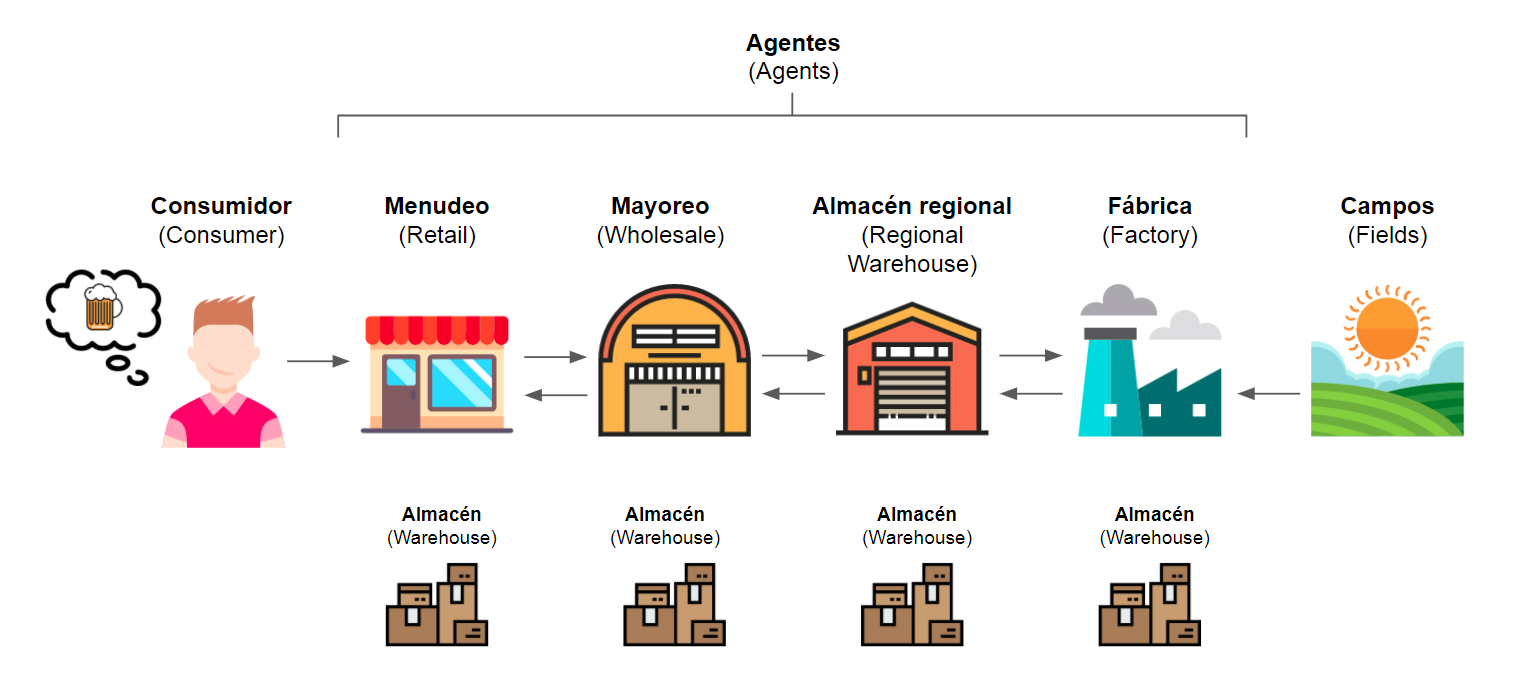
\includegraphics[width=15cm]{beer_distribution_game_structure.PNG}
\centering
\end{figure}

De esta manera, las variables que tienen efecto en este problema son:

\begin{itemize}
    \item Demanda del consumidor
    \item Producci\'on (oferta) de los campos
    \item Precio de la cerveza
    \item Costo de almacenaje
    \item Costo de oportunidad por \'ordenes no cumplidas
    \item Inventario inicial
\end{itemize}

Todas las variables, menos la demanda del consumidor y la producci\'on en los campos, pueden ser declaradas para el sistema (igual para todos los agentes) o individualmente (diferente para cada agente). Como se ver\'a m\'as adelante, el sistema es sumamente sensible a peque\~nos cambios en cualquiera de las variables; por ejemplo, si un agente comienza el juego con suficiente inventario para todo el a\~no, el agente superior nunca podr\'a venderle cerveza e incurrir\'a solamente en costos por almacenaje.

\subsection{El Efecto Látigo}

El \textit{Efecto Látigo} es un fen\'omeno que se produce en cadenas de suministro. Se llama de esa manera porque, mientras m\'as ``arriba'' en la cadena de suministro se encuentre un agente (es decir, m\'as lejos del contacto directo con el comprador), m\'as distorsionada es la informaci\'on que tiene acerca de la verdadera demanda del comprador; tal varianza se puede visualizar como una curva que asemeja un l\'atigo. \citet{Chaharsooghi} nota que la distorsi\'on se debe mayormente a tres factores: prejuicios en la informaci\'on de la demanda por parte de los miembros cercanos al consumidor, retraso en el intercambio de informaci\'on entre los miembros de la cadena y soporte log\'istico inapropiado a trav\'es de la cadena. \\

Se puede ejemplificar con el siguiente escenario:

\begin{enumerate}
    \item El consumidor, que generalmente compra $6$ cervezas, ahora quiere $10$, pero la tienda minorista solamente cuenta con $7$. El minorista le venderá todo su inventario, pues es la acci\'on que maximiza su ganancia. Despu\'es, debe decidir si volverá a tener un inventario de $6$ o si debe pedir un número mayor de cervezas, atendiendo la posible creciente demanda. Decide pedir $9$ cervezas al siguiente nivel, la tienda de mayoreo.
    \item El mayorista cuenta con $17$ cervezas. Llena el pedido del minorista, pero decide que ten\'ia guardado demasiado inventario, as\'i que se queda con $8$ cervezas en su almac\'en, sin hacer una orden al siguiente nivel, la tienda de distribución.
    \item La tienda de distribuci\'on decide no comprar unidades a la f\'abrica, dado que no disminuy\'o su inventario.
    \item La f\'abrica conoce la restricci\'on de estacionalidad de la cebada, as\'i que compra una m\'inima cantidad a los campos.
\end{enumerate}

En este escenario, el mayorista obtuvo informaci\'on distorsionada acerca del repentino crecimiento en la demanda del comprador, mientras que la tienda de distribución podr\'ia incluso interpretar que el comprador disminuy\'o su consumo. Si este comportamiento se mantiene durante algunos periodos m\'as, recibir\'ia la noticia (por medio de un incremento en las \'ordenes regulares) con un retraso considerable.\\

En el caso de que la demanda sea determinista (con un castigo por \'ordenes no cumplidas), la orden \'optima en cada tiempo para cada miembro de la cadena es ``una por una'', es decir, demandar al agente superior exactamente lo mismo que fue demandado por el agente inferior.

\subsection{La din\'amica de las existencias y flujos}

Las existencias y flujos (\textit{stocks and flows}) son componentes b\'asicos en un sistema din\'amico \footnote{Para mayor profundidad acerca de sistemas din\'amicos y el comportamiento de las existencias y flujos, \citet{Sterman} profundiza y provee de las bases adecuadas para sistemas m\'as complejos.}. Las existencias son acumulaciones basadas en la diferencia entre los flujos entrantes y los salientes. El flujo neto a una existencia en un tiempo determinado $t$ es la tasa de cambio de la existencia en el tiempo $t$:

$$
Existencia(t) = \int_{t_{0}}^t [Entrada(s) - Salida(s)]ds + Existencia(t_{0}) 
$$

Es com\'un que en un sistema con varias existencias con sus respectivos flujos ocurran retrasos. Esto sucede porque, en general, los flujos de entrada y salida son gobernados por decisiones diferentes. En el Juego de Distribuci\'on de Cerveza, para cada agente, su flujo de salida depende de la demanda del agente inmediatamente inferior limitada por su propia existencia, y su flujo de entrada depende de su propia demanda limitada por la existencia del agente inmediatamente superior. Esto, aunado a un comportamiento ligeramente aleatorio de la demanda del consumidor, puede desembocar en insuficiencia de existencias para cualquier agente en cualquier tiempo $t$. \\

Un capital est\'a en equilibrio cuando no cambia (un sistema est\'a en equilibrio cuando ninguna de sus existencias cambia). Esta condici\'on se obtiene cuando el cambio neto de sus flujos es cero, es decir, cuando el flujo entrante es igual al flujo saliente. \\

La soluci\'on trivial para este equilibrio es que todos los flujos sean nulos (\textit{equilibrio est\'atico}), sin embargo, en el caso de la cadena de suministro, este escenario llevar\'ia a que ning\'un agente tuviera ventas, y por consiguiente, tampoco tuviera ganancias. Una situaci\'on m\'as adecuada ser\'ia un \textit{equilibrio din\'amico}, en el cual las existencias totales se mantienen constantes, pero los flujos son diferences de cero\footnote{Para m\'as informaci\'on de un sistema en el cual se optimiza con base en se\~nales de baja existencia para disparar producci\'on, se puede consultar el proceso visual Kanban\cite{Majowska}}. Para la cerveza, esto significar\'ia que la cantidad de cerveza en los almacenes se mantiene constante, pero cada caja de cerveza se mueve de un agente a otro en alg\'un punto en el tiempo. Sin restricciones de oferta, la situaci\'on ideal tender\'ia a no guardar cerveza en los almacenes. Sin embargo, el efecto l\'atigo, causado por cambios en la demanda del consumidor, complica la estimaci\'on de los flujos entrantes y salientes en cada tiempo, pues para cada agente son desconocidas tanto la demanda del agente inferior como la capacidad del agente superior de cubrir la demanda propia. Existe una complicaci\'on extra al a\~nadir estacionalidad en la producci\'on de los campos de cebada. \\

\section{Acercamiento en el Presente Trabajo}

En este trabajo se modelará el Problema de Distribución de Cerveza, \textit{The Beer Distribution Game}, ampliamente utilizado y explicado por el Profesor \citet{Sterman} en la Escuela de Administraci\'on y Direcci\'on de Empresas Sloan del MIT, como una cadena de suministro, para ilustrar el concepto de \textit{efecto l\'atigo} (en ingl\'es, \textit{bullwhip effect}. Este efecto recibi\'o tal nombre debido a que la varianza en la informaci\'on acerca de la demanda real tiene el mismo comportamiento que un l\'atigo: mientras m\'as lejano se encuentra del origen (consumidor), mayor amplitud tiene la onda (varianza).\\

Existen acercamientos anteriores a este problema, en espec\'ifico \citet{Chaharsooghi} propone ya un acercamiento con \textit{Q-learning} \footnote{Los nombres de los algoritmos ser\'an representados con it\'alicas en este trabajo.} pero sin restricci\'on de estacionalidad en la materia prima, \citet{Strozzi}, por medio de Algoritmos Genéticos, \citet{Kimbrough} y \citet{Zarandi} proponen h\'ibridos de un algoritmo gen\'etico y aprendizaje reforzado.\\

Por otro lado, algunas l\'ineas de investigaci\'on como \citet{Busoniu} se han concentrado en el aspecto de teor\'ia de juegos que compete a este problema: si en un vendedor no tiene existencias, los consumidores podr\'an elegir otro. En este caso, los agentes son construidos como adversarios. Dado que en el modelo que se resuelve en el presente trabajo los agentes no son ni adversarios ni cooperativos, sino maximizan su propia utilidad, no se implementar\'a como este tipo de modelo.\\

Sin embargo, todos los acercamientos anteriores suponen que los campos pueden adaptarse de inmediato a la demanda de la f\'abrica, de cierta manera tienen "producci\'on infinita". El aporte de este trabajo es la imposici\'on de restricciones basadas en tendencias catalogadas por el departamento de agricultura de los EUA en la producci\'on de cebada, lo cual deber\'ia alterar el comportamiento de los agentes tal que mantengan una existencia positiva en sus almacenes para poder enfrentar la demanda en periodos de baja producci\'on.
